\documentclass{article}
\usepackage{geometry}
 \geometry{
 a4paper,
 left=40mm,
 top=20mm,
 }
\renewcommand{\baselinestretch}{1.2} 
\usepackage{graphicx}
\usepackage{subcaption}
\usepackage{amsmath}
\usepackage{authblk}
\usepackage{listings}
\usepackage{xcolor}
\lstset{
	language=C++,
    frame=tb, % draw a frame at the top and bottom of the code block
    basicstyle=\fontsize{9}{11}\selectfont\ttfamily, %font size
    tabsize=2, % tab space width
    showstringspaces=false, % don't mark spaces in strings
    commentstyle=\color{green}, % comment color
    keywordstyle=\color{blue}, % keyword color
    stringstyle=\color{red} % string color
}
\usepackage[ruled,vlined]{algorithm2e}

\begin{document}

\title{Continuum Mechanics II Project Report\\ 3D Panel Method \\}
\author{\small Andi Muhammad Zakiy Mukhlis (23619001) \\ Tobias Samuel Sugandi (23619009) \\ Muhammad Daffa Robani (23619020)}
\date{}
\affil{}
\maketitle

\hrule
\begin{abstract}

\end{abstract}
\hrule

\section{Introduction}

\section{Literature Review}

\section{Methodology}
\subsection{Geometry}
The calculation of panel surface is done by module of cross product of panel diagonals with following expression :
\begin{equation}
S = \frac{|\textbf{A}\times \textbf{B}|}{2}
\end{equation}
where $S$ is surface, $\textbf{A}$ and $\textbf{B}$ panel diagonals
\\ Calculation of collocation point $\textbf{c}$ is done by mean value of the panel coordinates :
\begin{equation}
c_x = \frac{x_1+x_2+x_3+x_4}{4} , c_y = \frac{y_1+y_2+y_3+y_4}{4} ,c_z = \frac{z_1+z_2+z_3+z_4}{4}
\end{equation}
where,$c_x,c_y,c_z$ are coordinates of collocation point of the panel and $x_i,y_i,z_i$ are coordinates of panel vertices 
\begin{figure}[ht]
	\centering
	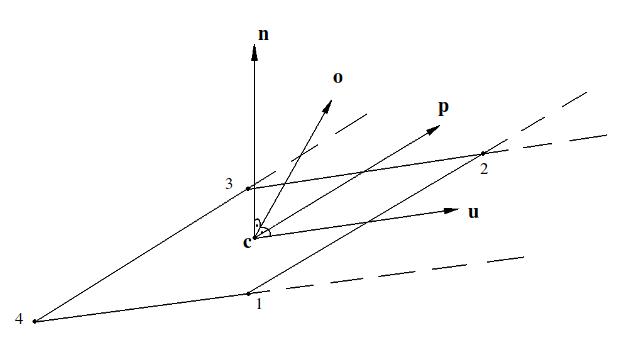
\includegraphics[width=100mm,scale=0.5]{panelvectors.png}
	\caption{Collocation point $\textbf{c}$ and unit vectors of panel}
	\label{fig:panelvector}
\end{figure}
\\ Calculation of unit vectors in longitudinal $\textbf{u}$ and transverse $\textbf{p}$ direction is performed by :
\begin{align}
u_x = \frac{x_1+x_2-x_3-x_4}{2},u_y = \frac{y_1+y_2-y_3-y_4}{2},u_z = \frac{z_1+z_2-z_3-z_4}{2}
\\ p_x = \frac{x_2+x_3-x_1-x_4}{2},p_y = \frac{y_2+y_3-y_1-y_4}{2},p_z = \frac{z_2+z_3-z_1-z_4}{2}
\end{align} 
\\ Calculation of unit vector perpendicular to the unit vectors $\textbf{n}$ and $\textbf{u}$ is done by $\textbf{o}=\textbf{n}\times \textbf{u}$
\\ 
%\begin{algorithm}[H]
%\SetAlgoLined
%\KwIn{Wing and Flap Chord ($c$ and $cf_c$), \\
% \qquad \qquad , \\
% \ForEach{Panel}{
%	  \;
%	  \;
% }
% \caption{Structured Grid}
%\end{algorithm}

\section{Result and Discussion}
\subsection{Result}
%\begin{figure}[h]
%	\centering
%	\includegraphics[width=\linewidth]{Result1.png}
%	\caption{Results 1}
%	\label{fig:g1}
%\end{figure}

\subsection{Discussion}

\section{Conclusions}
\begin{itemize}
\item 
\end{itemize}

\section{References}

\begin{itemize}
    \item 
\end{itemize}

\section{Numerical Code}
\begin{lstlisting}[title={}]

\end{lstlisting}
\end{document}